\chapter{Wstęp}
\label{sec:description}
	\section{Cel}
	Celem pracy inżynierskiej jest budowa środowiska symulacyjnego robota mobilnego z kołami szwedzkimi.
	Dla realizacji tego celu należy opracować model 3D, oraz model dynamiki dookólnej bazy jezdnej z 4 kołami szwedzkimi.
	Jednym z przyjętych założeń jest wymaganie, aby opracowany model był możliwie dokładny i jego działanie było zbliżone do rzeczywistego robota.
	Opisywana platforma będzie używana jako baza wielokierunkowa do przemieszczania dwuramiennego robota manipulacyjnego Velma.

	Celem jest stworzenie modelu, który będzie reagował na siły podobnie do rzeczywistego robota i był sterowany tak samo, jak rzeczywisty robot.
	To spowoduje, że możliwe będzie stworzenie jednego wspólnego programu sterującego, do użycia zarówno w symulacji, jak i rzeczywistym robocie.

	Testowanie oprogramowania sterującego na rzeczywistym obiekcie może prowadzić do jego uszkodzeń, 
	dlatego wpierw należy się upewnić o poprawności projektowanych rozwiązań na bezpiecznym modelu wirtualnym.
	Rzeczywistość nie pozwala także na skomplikowane scenariusze testów, które w rzeczywistości mogłyby być niemożliwe do wykonania lub koszty jego wykonania byłyby zbyt wysokie.
	Szybciej i taniej jest stworzyć symulacyjne środowisko testowe, niż fizyczne, w dodatku błąd sterowników przy symulacji nie grozi zniszczeniem rzeczywistego robota.
	Dopiero przy osiągnięciu satysfakcjonującej jakości sterowania w symulacji wirtualnej, 
	można zastosować algorytmy sterowania do rzeczywistego obiektu bez ryzyka uszkodzeń urządzenia.

	Oprócz modelu bazy jezdnej, środowisko symulacyjne musi również udostępniać modele czujników, w które wyposażony jest robot. 
	Odczyty z symulatorów czujników są następnie wykorzystywane w układzie sterowania do generacji odpowiednich sygnałów sterujących.
	W celu możliwie wiernej symulacji działania czujników, do wartości pomiarów dodaje się szum pomiarowy i zakłócenia.

\section{Składniki systemu}
	Środowisko symulacyjne składa się z kilku odrębnych modułów, które komunikują się ze sobą poprzez specjalne interfejsy, wykorzystujące kolejki wiadomości.
	Taka implementacja komunikacji pozwala zmieniać i reimplementować poszczególne elementy i używać różnych języków programowania, 
	zachowując jednolitą komunikację między składnikami i nie tracąc na kompatybilności między komponentami.
	Możliwe jest także przesyłanie wiadomości przez sieć, co pozwala na rozproszenie systemu.

	%TODO Zmienić na Tikz
	\begin{figure}[H]
	\centering
	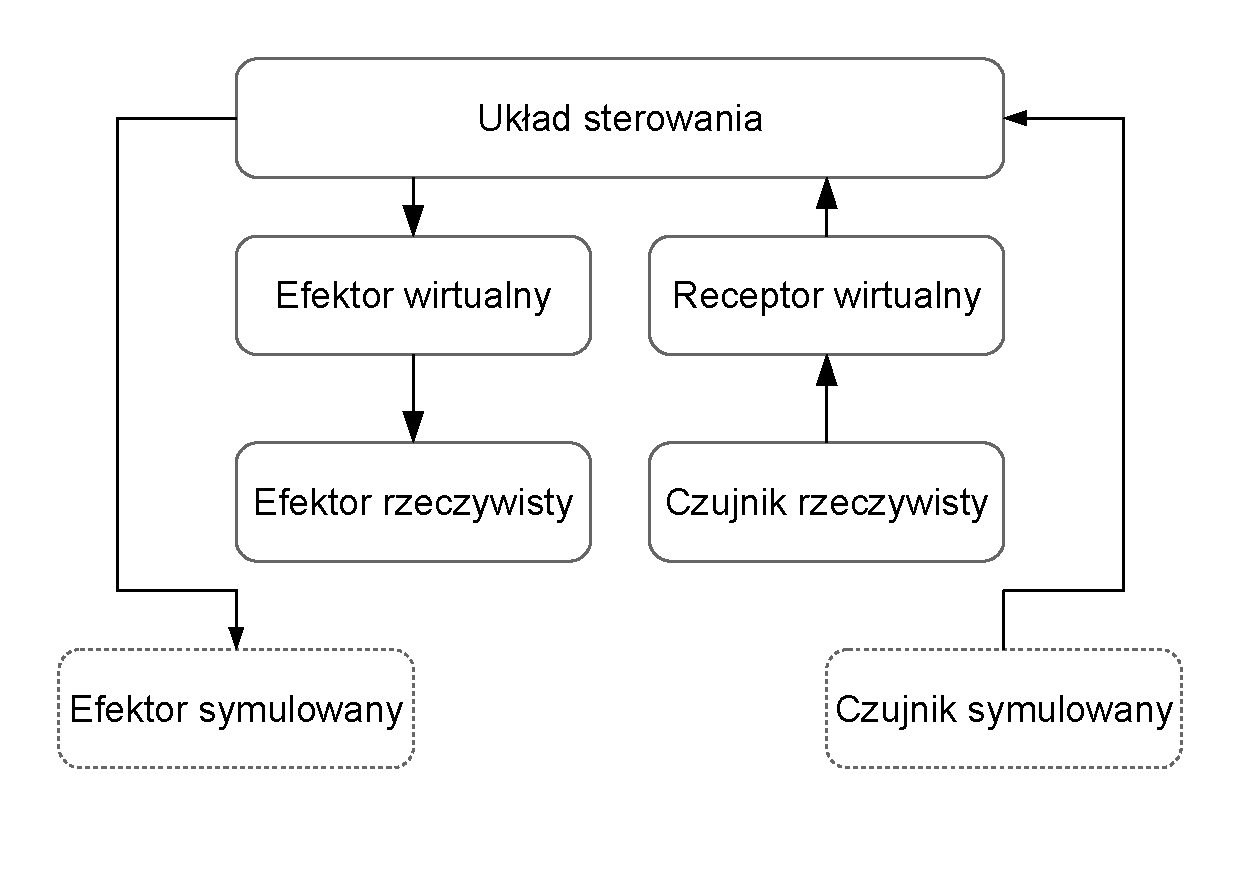
\includegraphics[width=0.8\textwidth]{graphics/agent.pdf}
	\caption{Struktura agenta upostaciowionego.}
	\label{fig:agent}
	\end{figure} 

	Można to przedstawić za pomocą zapisu agentowego, rysunek \ref{fig:agent}.
	Agent upostaciowiony składa się z kilku modułów, komunikujących się ze sobą za pomocą różnych interfejsów.

	Nadrzędnym modułem jest układ sterowania, który na podstawie odczytów z czujników generuje sterowanie dla efektorów.
	Ważne jest, aby komunikacja z rzeczywistymi urządzeniami była identyczna, jak z ich modelami, dzięki czemu taki system będzie przenośny i niezależny od implementacji modelu.

	Efektor rzeczywisty, na przykład serwomotor, jest sterowany za pomocą efektora wirtualnego, który zamienia wyjście układu sterowania na sygnały sterujące dla silnika napędowego.
	Przykładowo, zmienia odebraną liczbę, oznaczającą zadaną prędkość, na odpowiednie napięcie na wyjściu układu sterującego.

	Zamodelowany efektor symulowany również przyjmuje te same sygnały do układu sterowania, co efektor rzeczywisty, 
	lecz nie zamienia ich na sygnały sterujące, a wywołuje odpowiednie funkcje maszyny symulacyjnej, nadające siły i prędkości obiektom w przestrzeni wirtualnej.

	Receptor wirtualny pobiera surowe dane z czujnika, przekształca na odpowiedni format, usuwa błędy i szum tak, aby program sterujący mógł wykorzystać te dane w prosty sposób. 
	Doskonałym przykładem jest tutaj urządzenie Kinect (widoczne na robocie Velma na fotografii \ref{fig:velma}), w którym to zachodzi odczytanie obrazu z kilku kamer.
	Następnie obraz przesyłany jest do komputera, w którym sterowniki interpretują dane, usuwając błędy, tworzą mapę głębokości, wykrywają szkielety i sylwetki osób.
	Te dane mogą być wykorzystane łatwo w grach i programach sterujących.

	Modelowanie receptora, tak jak w przypadku efektora, polega na wygenerowaniu odpowiednich danych, używając odpowiednich funkcji w przestrzeni wirtualnej.
	Mogą one polegać na emitowaniu półprostych, symulujących laser, lub wręcz renderowaniu obiektów, aby uzyskać obraz z wirtualnej kamery.
	Receptor symulowany ma pełną wiedzę o symulowanym świecie, dokładne pozycje i prędkości wszystkich obiektów, dane o kolizjach itp. 
	Pozwala to na łatwe symulowanie receptorów nie mogących mieć odwzorowania w rzeczywistości, co przydatne jest w pierwszych stadiach testowania i wyznaczaniu statystyk.
	Takim przykładem jest model czujnika dokładnej pozycji, rotacji i prędkości w kartezjańskim układzie współrzędnych. 
	Czujniki typu GPS, lub żyroskopy nie generują tak dokładnych pomiarów.

	\subsection{Model 3D}
		Model 3D bazy mobilnej, opisany równaniami matematycznymi, powinien mieć zachowanie zbliżone do oryginału, najbardziej jak to tylko możliwe.
		Musi uwzględniać masy i momenty bezwładności elementów składowych, a także wszystkie tarcia.
		Model obejmuje więzy na ruchome elementy, takie jak koła i rolki, aby umożliwić symulację przegubów.

		Model składa się z elementów, odwzorowujących rzeczywiste części składowe bazy mobilnej.
		Elementy posiadają takie cechy, jak:
		\begin{itemize}
			\item Pozycja w modelu.
			\item Masa.
			\item Moment bezwładności.
			\item Kształt fizyczny.
			\item Materiał fizyczny.
			\item Wygląd.
		\end{itemize}

		Dodatkowo, należy uwzględnić wszystkie więzy, w postaci symulowanych przegubów.
		W przypadku tej bazy istnieje typ więzów o jednym stopniu swobody (zawias), używany przy połączeniu przedniej i tylnej części platformy, oraz 
		jako piasty kół i rolek. Można także uznać, że więzy bez stopni swobody używane są do trwałego połączenia czujników z platformą i transportowanym robotem.
		Więzy mogą oddziaływać siłą na elementy do których są podłączone, symulując silniki.

		Elementy składowe i symulowane przeguby oddziałują bezpośrednio z maszyną do symulacji fizycznej. 
		To kształt, masy i momenty bezwładności brył są argumentami funkcji liczących.
		Maszyna symulacyjna oblicza odpowiednie prędkości i nadaje je podanym obiektom w podobny sposób, jak ma to miejsce w rzeczywistości.

		Do modelu doczepia się wirtualne czujniki, generujące odpowiednie dane na podstawie symulacji i rozkładu losowego.
		Nie są to pełne dane o stanie modelu, jakie posiada maszyna do symulacji, gdyż czujniki fizyczne również nigdy nie mają pełnej informacji o stanie urządzenia.
		Należy dodać losowy szum i błędy, aby przybliżyć ich zachowanie do rzeczywistych czujników.

		Dla ozdoby, można wykorzystać istniejący model CAD do stworzenia siatki trójwymiarowej i nadania symulowanemu obiektowi wyglądu zbliżonego do fizycznego robota.

	\subsection{Sterownik silników}
		Program sterujący generuje abstrakcyjne dane, na przykład liczbę zmiennoprzecinkową, zapisaną binarnie.
		Przykładowy silnik fizyczny nie jest w stanie działać na podstawie takich danych, do pracy potrzebuje odpowiedniego napięcia na wejściu,
		ale interfejs serwomotoru na przykład przyjmuje bardziej abstrakcyjne dane w formie liczby stałoprzecinkowej, jako pole w odebranej ramce.
		Do tłumaczenia jednych danych na drugie, potrzebny jest sterownik niskopoziomowy.
		Najczęściej implementowany jest w formie mikrokontrolera, lub podobnego systemu wbudowanego.

		Jego zadanie to odczytanie danych, podanych przez program sterujący i na przykład generowanie na ich podstawie odpowiedniego przebiegu PWM, lub obsługa przetwornika cyfrowo-analogowego.
		Do innych zadań może należeć kontrola, czy żądana wartość nie uszkodzi urządzenia.
		Zazwyczaj sterownik może komunikować się z powrotem z resztą systemu, aby zgłaszać ewentualne awarie.

		Taki program i powiązany z nim układ elektroniczny są najczęściej dostarczone przez producenta robota i nieznane użytkownikowi.
		Dodatkowo, tworzy to kolejną warstwę abstrakcyjną dla sterownika głównego, który nie musi zważać na generowanie różnych danych dla różnych modeli tych samych efektorów.
		
		W środowisku wirtualnym należy stworzyć moduł o podobnym działaniu.
		Powinien przyjmować dane w dokładnie takim samym formacie, jak opisany wyżej układ, aby był łatwo wymienialny na sterownik fizycznego urządzenia bez ingerencji w główny program sterujący.
		Zamiast zamieniać odczytane dane na analogowe wartości, on wywołuje odpowiednie funkcje maszyny symulacyjnej, aby wywołać taki sam efekt, co na rzeczywistym efektorze, lecz w wirtualnej przestrzeni symulacji.
		Jako argumenty podaje parametry fizyczne symulowanego obiektu, oraz przyłożone siły.
		

	\subsection{Sterownik czujników}
		Implementowany podobnie do sterownika silników, ma za zadanie konwertować surowe i obarczone błędami dane z czujników, na format zrozumiały dla programu sterującego.
		W tym miejscu usuwa się błędy grube, niweluje stałe na podstawie kalibracji, wygładza szum i interpretuje dane, aby pozyskać wymagane przez wyższe warstwy informacje.

		Przykładowo, czujniki laserowe zwracają jedynie ciąg pomiarów, ale to do tego programu należy interpretacja wykrytych kształtów, łączenie punktów i obróbka do formatu zrozumiałego dla wyższych podzespołów.
		Większość zaawansowanych receptorów posiada owe układy cyfrowe i programy wbudowane w urządzenie.
		Dostarczone są przez producenta tak samo, jak sterowniki efektorów.
		
		Aby zasymulować ten element, należy zbudować program generujący dane na podstawie aktualnego stanu maszyny do symulacji, w sposób w jaki działa czujnik w rzeczywistości.
		Na przykład, dla czujnika laserowego, silnik symulacji fizycznej emituje odpowiednią ilość promieni i oblicza ich punkty przecięcia się z wirtualnymi modelami.
		Renderowanie obrazu pozwala na symulację kamery.

		Ponieważ dane fizyczne nigdy nie są idealne, w celu przybliżenia wyjścia wirtualnego czujnika do oryginału, dodaje się szum o odpowiednim rozkładzie i błędy.

	\subsection{Program sterujący}
		W programie sterującym obliczane jest sterowanie, na podstawie dostarczonych odczytów z czujników.
		Zazwyczaj wykorzystuje się tutaj także zewnętrzne biblioteki, dostarczające zaawansowane algorytmy.
		Ich zadania mogą polegać na budowie wewnętrznej mapy, wyznaczaniu ścieżki, omijaniu przeszkód, odwrotnej kinematyce i tym podobnych.

		Taki program zwykle działa na mocniejszych układach logicznych, niż sterowniki, ze względu na duże zapotrzebowania na moc obliczeniową
		i niedeterministyczny czas obliczeń.
		Jeśli robot komunikuje się z użytkownikiem, to zachodzi to w tym module. 

		Programy sterujące mogą być implementowane w językach wysokopoziomowych, nawet skryptowych, gdyż wymagania czasowe nie są rygorystyczne.
		Co więcej, często się zdarza, że odpowiednie składowe programu bazują na różnych technologiach.

		Środowisko symulacyjne powinno zapewnić pełną abstrakcję komunikacji tego modułu.
		Oznacza to, że niezależnie, czy program steruje rzeczywistym robotem, czy symulacją wirtualną, zawsze powinien móc komunikować się i otrzymywać dane w tym samym formacie.
		W idealnym przypadku program nie powinien mieć możliwości stwierdzić, czy steruje symulacją, czy fizycznym urządzeniem.
		
\section{Plan pracy}
	\begin{enumerate}
	\item Należy stworzyć model platformy do uruchomienia w symulatorze, zachowując wszystkie rozmiary i momenty rzeczywistej wersji.
	Bryły składowe modelu muszą przypominać kształtem części z których składa się robot, należy im także ustawić parametry fizyczne, jak masę, moment bezwładności, materiał itp.
	\item Zamodelowanie wszystkich więzów na koła, rolki i przegub, aby maszyna symulacyjna poprawnie symulowała obiekt.
	Taki model powinien na tym stanie poprawnie reagować na wirtualne siły, lecz jego efektory nie będą jeszcze aktywne.
	Można go prosto pobieżnie przetestować działając siłą na elementy i patrząc, czy reagują w spodziewany sposób.
	\item Zapisanie wtyczki sterującej modelem, odczytującej odpowiednie dane z zewnątrz i wywołującej funkcje maszyny symulacyjnej, aby modyfikować ruch modelu.
	Na tym poziomie można dobudować zamiennik programu sterującego, jedynie do podawania prostych wartości bez odczytywania pomiarów i sterowania.
	\item Stworzenie modelu kinematycznego, aby przetestować, czy model dynamiczny zachowuje się w miarę poprawnie.
	\item Zaprogramowanie wtyczki symulującej podstawowe czujniki, aby generowały dane z enkoderów, oraz innych urządzeń, dodawały błędy pomiarowe, a następnie przekształcały dane na format zrozumiały dla programu sterującego.
	Czujniki nie muszą być istniejące, mogą generować dane, jak pozycja i rotacja, bardzo trudne do uzyskania rzeczywistymi czujnikami.
	\item Wystawienie do zmiany w czasie rzeczywistym masy, momentu bezwładności, współczynników tarcia, aby pozwolić na proste testowanie działania systemu z różnymi współczynnikami.
	\item Elementy pomagające w symulacji, jak model kinematyki odwrotnej, sterowany funkcją matematyczną, i podłoże ze zmiennym współczynnikiem tarcia.
	\item Programy pomocnicze, zbierające i wyświetlające dane, interfejs graficzny do prostego sterowania robotem.
	\item Model czujnika laserowego, powinien zbierać dane i przekazywać je dalej. Musi posiadać także określone kształty.
	\item Model czujnika inercji, może być w pełni zaimplementowany jako program.
	\item Uproszczony program sterujący, aby zbadać, czy system działa poprawnie na tyle, aby rozwinąć go w końcowy projekt.
	\item Program sterujący w ROS. Największy i najbardziej skomplikowany element, wspólny dla obu bytów --- wirtualnego i rzeczywistego.
	Zwykle nie jest to praca jednego człowieka, a jego rozwój nie ustaje przez długi czas.
	Ten program dostarczy funkcji, aby wyższy sterownik robota mógł użyć tego modułu do sterowania jazdą i odczytywania danych.
	\end{enumerate}
	
\section{Istniejące implementacje}
	Istnieją także inne modele jeżdżących robotów na kołach szwedzkich.
	Można z nich brać przykład i sugerować się źródłami kodu i budową modeli.

	Kuka Youbot jest popularnym robotem wielokierunkowym. Jego modele są domyślnie dostępne w różnych symulatorach, między innymi w Gazebo i V-Repie, które są dobrymi kandydatami do 
	użycia w projekcie.
	Tylko w przypadku V-Repa, istnieje wstępny sterownik do którego da się wysyłać odpowiednie wartości kierunku, a on nadaje takie prędkości kołom, aby poruszać modelem w zadanym kierunku.
	Wersja dla Gazebo jest statycznym obiektem z błędnie ustanowionymi przegubami, jego efektory nie są zaimplementowane.
	
	Dodatkowo, V-Rep posiada wbudowane dwa inne pojazdy o napędach kół Mecanum i czujnikach laserowych.
	Zewnętrzne modele także pomogą przy wstępnej weryfikacji zachowania się budowanego tutaj modelu, czy nie zachowuje się nadzwyczaj dziwnie w pierwszych fazach projektu.

	Ze względu na niezwykle zaawansowany obiekt kół i kształt rolek, ważne jest aby uprościć model, poprzez zamianę niektórych składowych i dodanie sztucznych więzów.
	Całościowy model może być zbyt skomplikowany, aby maszyny symulacji mogły go obliczać w czasie rzeczywistym.
	Dokładny model także jest znacznie trudniej poprawnie wymodelować, ze względu na liczne tarcia i poślizgi rolek.
	Proponowane uproszczenia modeli opisane są w sekcji \ref{sec:omnivelma}.
	
\section{Podział tej pracy na sekcje}
	Kolejne rozdziały kolejno opisują różne aspekty pracy.
	\begin{description}
		\item[\nameref{sec:description}] Ten rozdział, zawiera ogólny opis pracy i sposób jej wykonania.
		\item[\nameref{sec:tools}] Opis narzędzi programistycznych, użytych przy budowie modeli i testowaniu.
		\item[\nameref{sec:robot}] Techniczny opis rzeczywistej platformy i czujników, oraz mechaniki stojącej za zasadą ich działania.
		\item[\nameref{sec:model}] Implementacje modeli opisanych w poprzednim rozdziale, problemy i niedoskonałości z nimi związane.
		\item[\nameref{sec:components}] Opis poszczególnych dodatkowych składników systemu, używanych w symulacji, testowaniu, wizualizacji i wspomagających tworzenie.
		\item[\nameref{sec:tests}] Testy różnych składników systemu, wykresy, interpretacja i podsumowanie.
	\end{description}
